%!TEX root = ../dissertation.tex
\begin{savequote}[75mm]
Knowledge knows no bounds.
\qauthor{Creator}
\end{savequote}

\chapter{Motivation and Theory}
%\newthought{There's something out there that we don't know.} 

%%%%%%%%%%%%%%%%
\section{The Standard Model and the Higgs Boson}
\paragraph{}
The Standard Model(SM) ~\cite{Pdg,Griffiths,Tully,Schwartz} is a quantum field theory describing the interactions of fundamental particles. The partciles are shown in Figure~\ref{fig:SM}. So far, the SM predictions agree extremely well with experimental observations.

\begin{figure}[h!]
  \centering
  \captionsetup{justification=centering}
  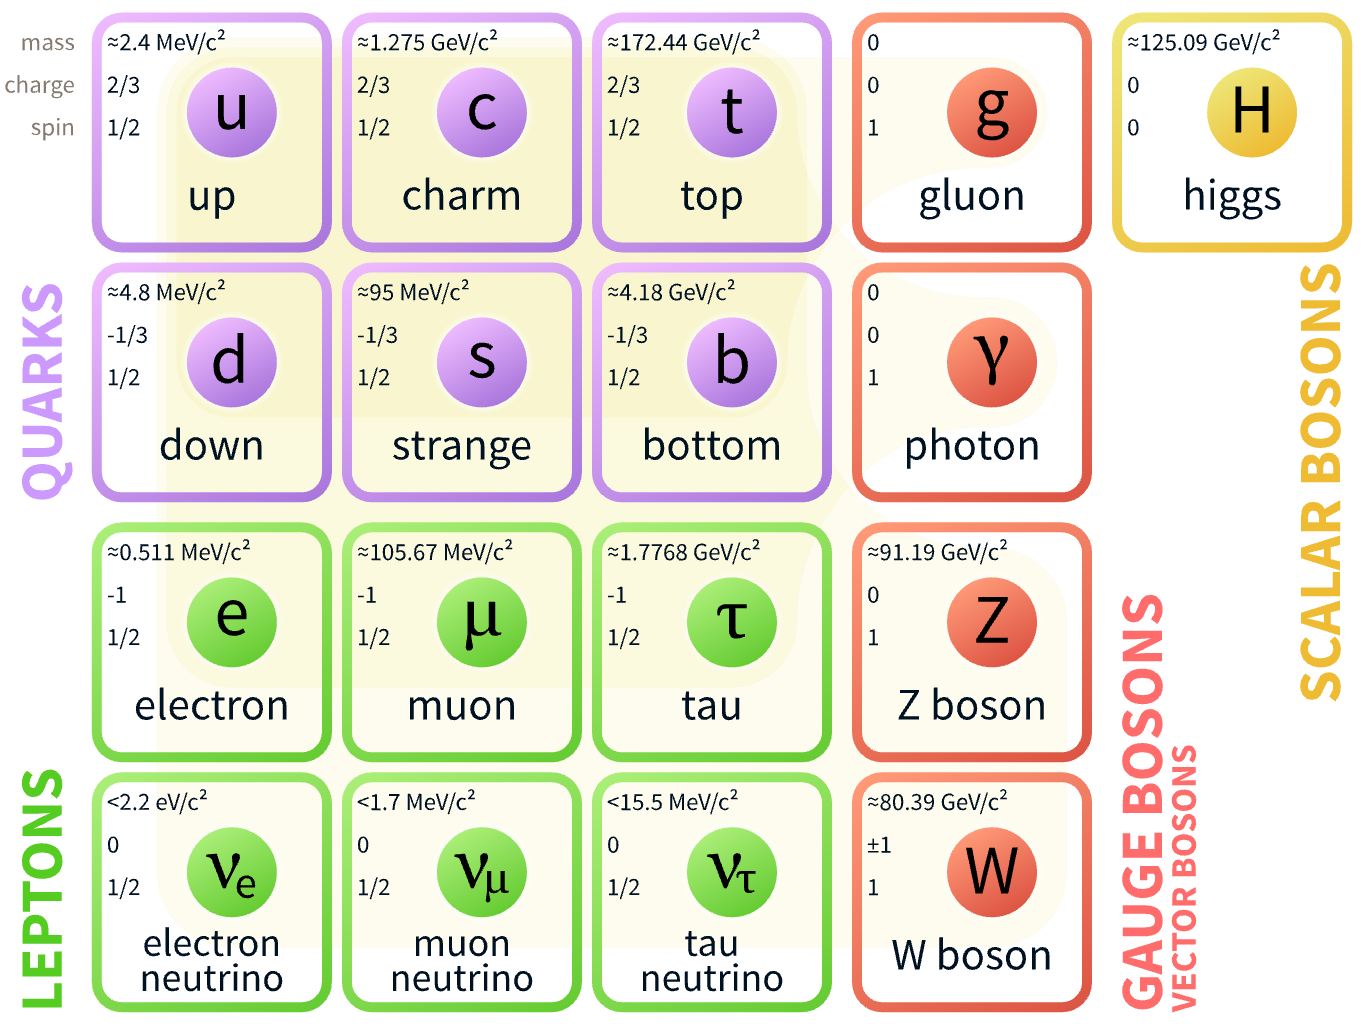
\includegraphics[width=0.6\textwidth]{figures/theory/SM}
  \caption{Fermions and bosons of the Standard Model and their properties~\cite{Pdg}, where all the values are measured experimentally.}
  \label{fig:SM}
\end{figure}

\paragraph{}
%However, in SM, due to the gauge invriance under $SU(2)_{L}$, fermions have to be massless in order to have pure left handed states. 
%The bosons must also be massless as required by the gauge principle. 
In the SM, the Higgs mechanism introduces a complex scalar Higgs field, $\phi$, with nonzero vacuum expectation values. Through spontaneous symmetry breaking of the Higgs potential $V(\phi) = -\nu^2\lambda_{\rm \nu} \phi^{\dagger}\phi + \lambda_{\rm \nu}(\phi^\dagger\phi)^2$, $W^{\pm}$ and $Z$ bosons acquire their masses. This process also predicts an extra scalar, the Higgs boson. The SM Lagrangian containing Higgs couplings, $\mathcal{L}_{\rm Higgs}$, is shown in Eq~\ref{eqn:higgspotential}.
\begin{equation}
\label{eqn:higgspotential}
% V(\phi_{h}) = \lambda \nu^2 \phi_{h} ^2  + \lambda \nu \phi_{h} ^3  + \frac{1}{4}\lambda \phi_{h} ^4 
\mathcal{L}_{\rm Higgs} = -\lambda_{hf\bar{f}} hf\bar{f} + \delta_{V} V_{\rm\mu} V^{\rm\mu}\left(\lambda_{\rm hVV} h + \lambda_{\rm hhVV}h^2\right) + \lambda_{\rm hh}h^2 + \lambda_{\rm hhh}h^3 + \lambda_{\rm hhhh}h^4 
\end{equation}
where 
\begin{itemize}
	\item $\rm\nu \sim 246$ \GeV, is the non-zero expectation value of the Higgs field;\
	\item $m_{\rm h} = \sqrt{2\lambda_{\rm \nu}}\nu \sim 125$ \GeV, is the Higgs mass; this is discovered in 2012\cite{ATLASHiggsDisc, CMSHiggsDisc}; 
	\item $\lambda_{\rm \nu}$, coefficient for the quartic potential term, is constrained from Higgs mass, to be $\sim 0.13$;
	\item $V = W^{\pm}$ or $Z$, $\delta_{W} = 1$, $\delta_{Z} = \frac{1}{2}$;
	\item $\lambda_{hf\bar{f}} = \frac{m_{\rm f}}{\rm\nu}$, is the Higgs to fermion coupling; $m_{\rm f}$ is the mass of the fermion;
	\item $\lambda_{\rm hVV} = \frac{2m_{\rm V}^2}{\rm\nu}$, is the Higgs to boson coupling; $m_{\rm V}$ is the mass of the boson;
	\item $\lambda_{\rm hhVV} = \frac{m_{\rm V}^2}{\rm\nu^2}$, is the Higgs-Higgs to boson-boson coupling;
	\item $\lambda_{\rm hh} = \frac{m_{\rm h}^2}{2}$, is the Higgs mass term;
	\item $\lambda_{\rm hhh} = \frac{m_{\rm h}^2}{2\rm\nu} = \lambda_{\rm \nu} \nu$, or $\lambda_{\rm hhh}$, is the Higgs self-coupling;
	\item $\lambda_{\rm hhh} = \frac{m_{\rm h}^2}{8\rm\nu^2}$, is the Higgs quartic-coupling.
\end{itemize}
\paragraph{}
What's particularly interesting and has not been measured experimentally in Eq~\ref{eqn:higgspotential} is $\lambda_{\rm hhh}$. SM predicts $\lambda_{\rm hhh} = \frac{m_{\rm h}^2}{2\rm\nu}$, which is referred as \textbf{$\lambda_{\rm SM}$} in this thesis. This term directly probes the Higgs potential.
%A different coupling from $\lambda_{\rm SM}$ is usually referred as just $\lambda$. 
Also, $\lambda_{\rm hhh}h^3$ term shows one way for double Higgs production within the SM. Double Higgs production is also known as \textbf{di-Higgs or Higgs pair production}.

%Di-Higgs final states will provide complementary information from single Higgs physics at the LHC.
%Measuring this coefficient is one of the major tasks of experimental particle physics program.

%%%%%%%%%%%%%%%%
\section{Standard Model di-Higgs production}

% \begin{figure}[h!]
%   \centering
%   \captionsetup{justification=centering}
%   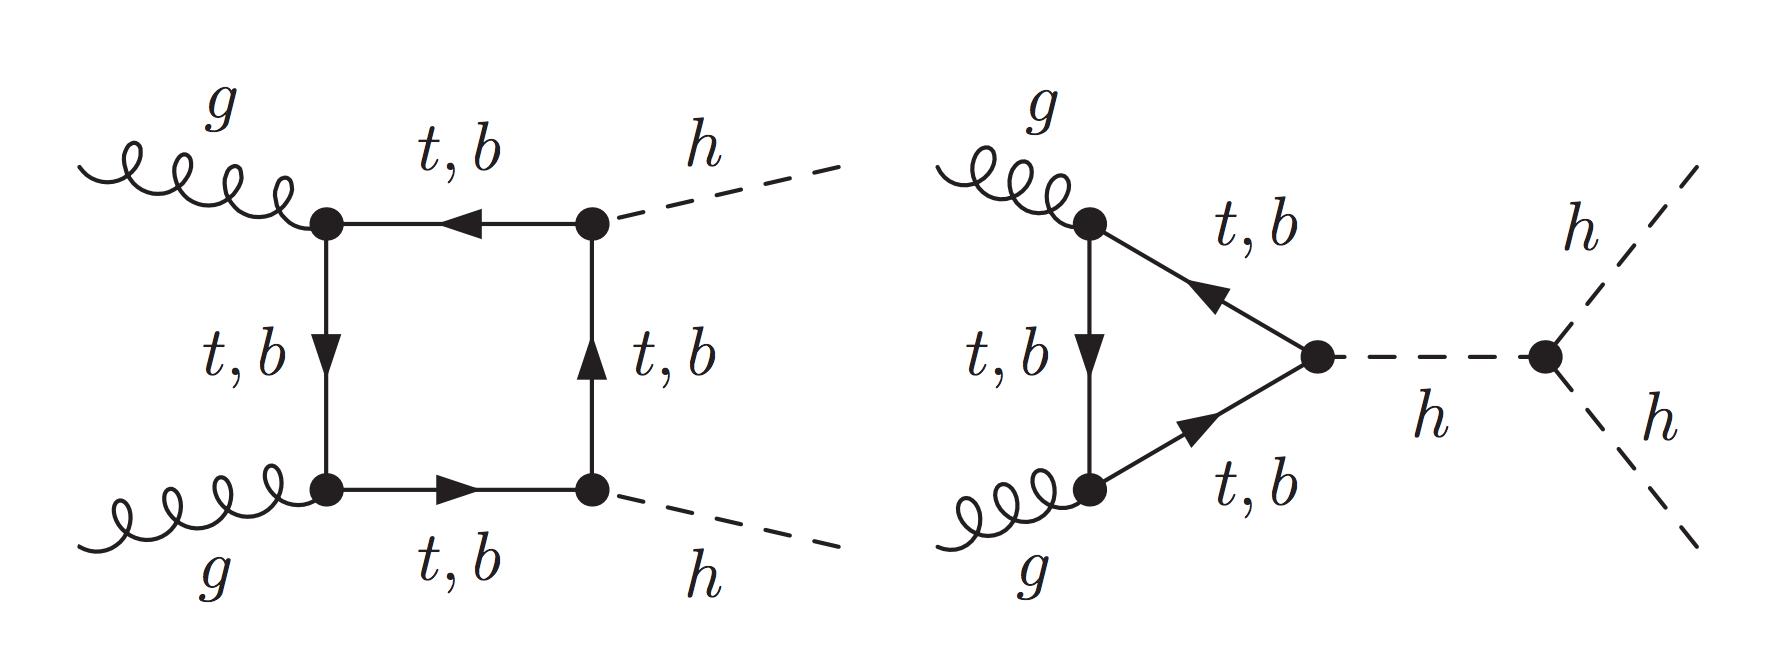
\includegraphics[width=0.7\textwidth]{figures/theory/SM_HH}
%   \caption{Feynman diagrams contributing to di-Higgs production via gluon-gluon fusion, through a $t$ or $b$ quark loop, at leading order. Only the right hand plot probes $\lambda_{hhh}$.}
%   \label{fig:SM_HH}
% \end{figure}

% \paragraph{}
% In the SM, the Higgs boson pair production through the $\lambda_{\rm hhh}$ has an on-shell component and a large off-shell component. The on-shell is strongly disfavored, requiring two off-shell Higgs bosons in the final state. The sensitivity region to the trilinear coupling production as in ~\ref{fig:SM_HH_tri}, is mainly in the kinematic region where the two Higgs boson in the final state are on-shell and the Higgs boson acts as a propagator (off-shell).

\paragraph{}
There are two main production diagrams of di-Higgs at the LHC, shown in Figure~\ref{fig:SM_HH}. In the gluon-gluon  fusion process, di-Higgs are produced through a box or a triangle loop. Only the triangle loop~\ref{fig:SM_HH_tri} probes the $\lambda_{hhh}$. In the triangle diagram, the middle Higgs boson acts as a propagator (off-shell), and the two Higgs boson in the final state are on-shell. An on-shell middle Higgs, with two off-shell Higgs bosons in the final state, is strongly disfavored~\cite{Pdg}. The box and triangle diagrams interfere destructively, which makes the overall production rate smaller than what would be expected in the absence of a $\lambda_{hhh}$ term.

\begin{figure}[h!]
\centering
\captionsetup{justification=centering}
    \begin{subfigure}[b]{0.4\textwidth}
        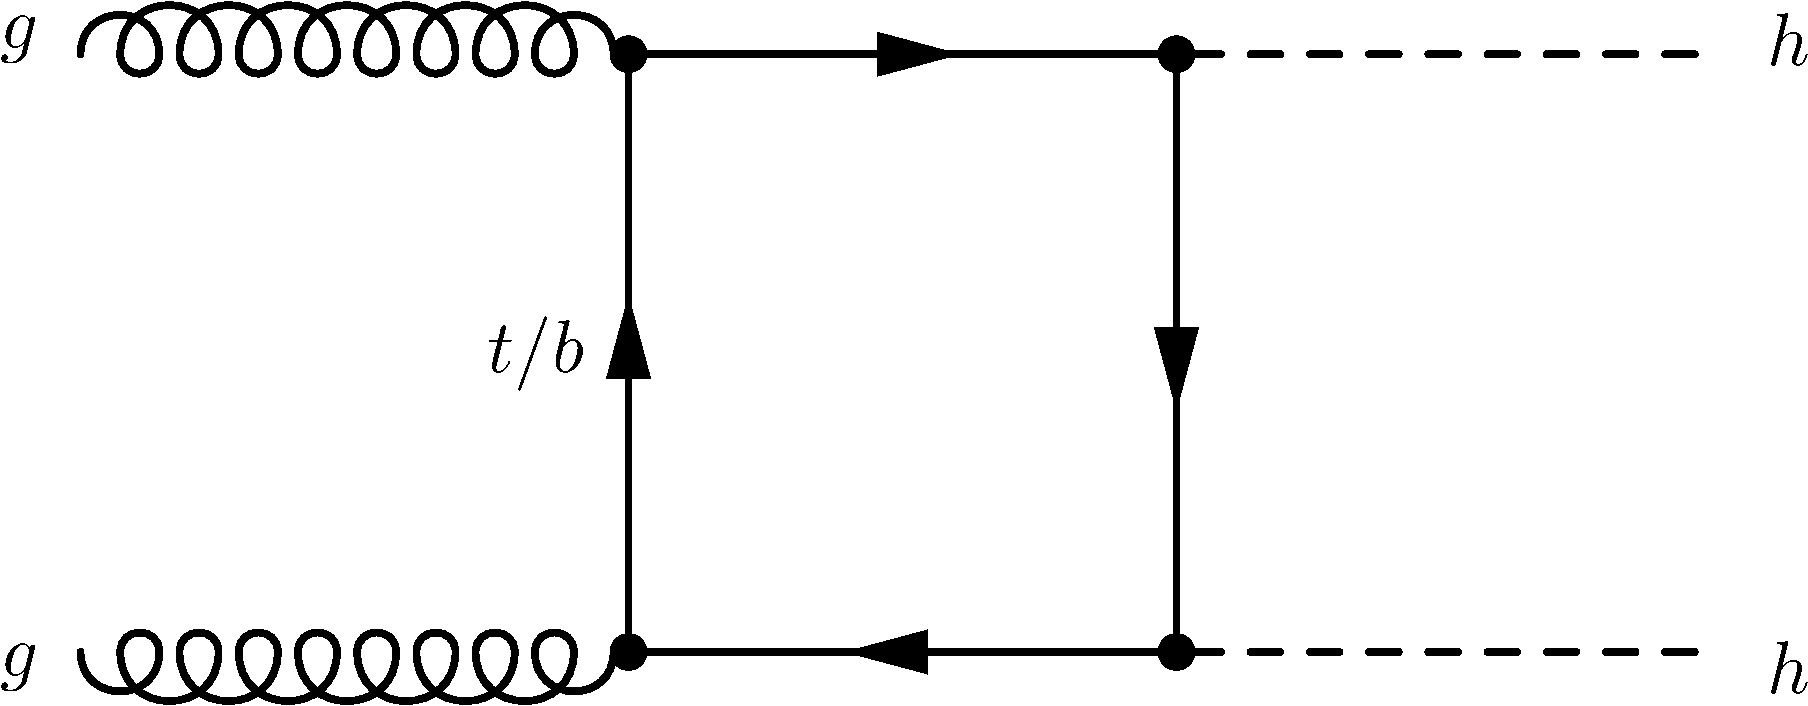
\includegraphics[width=\textwidth]{figures/theory/SM_HH_box}
        \caption{Box diagram}
        \label{fig:SM_HH_box}
    \end{subfigure}
    \quad
    \begin{subfigure}[b]{0.4\textwidth}
        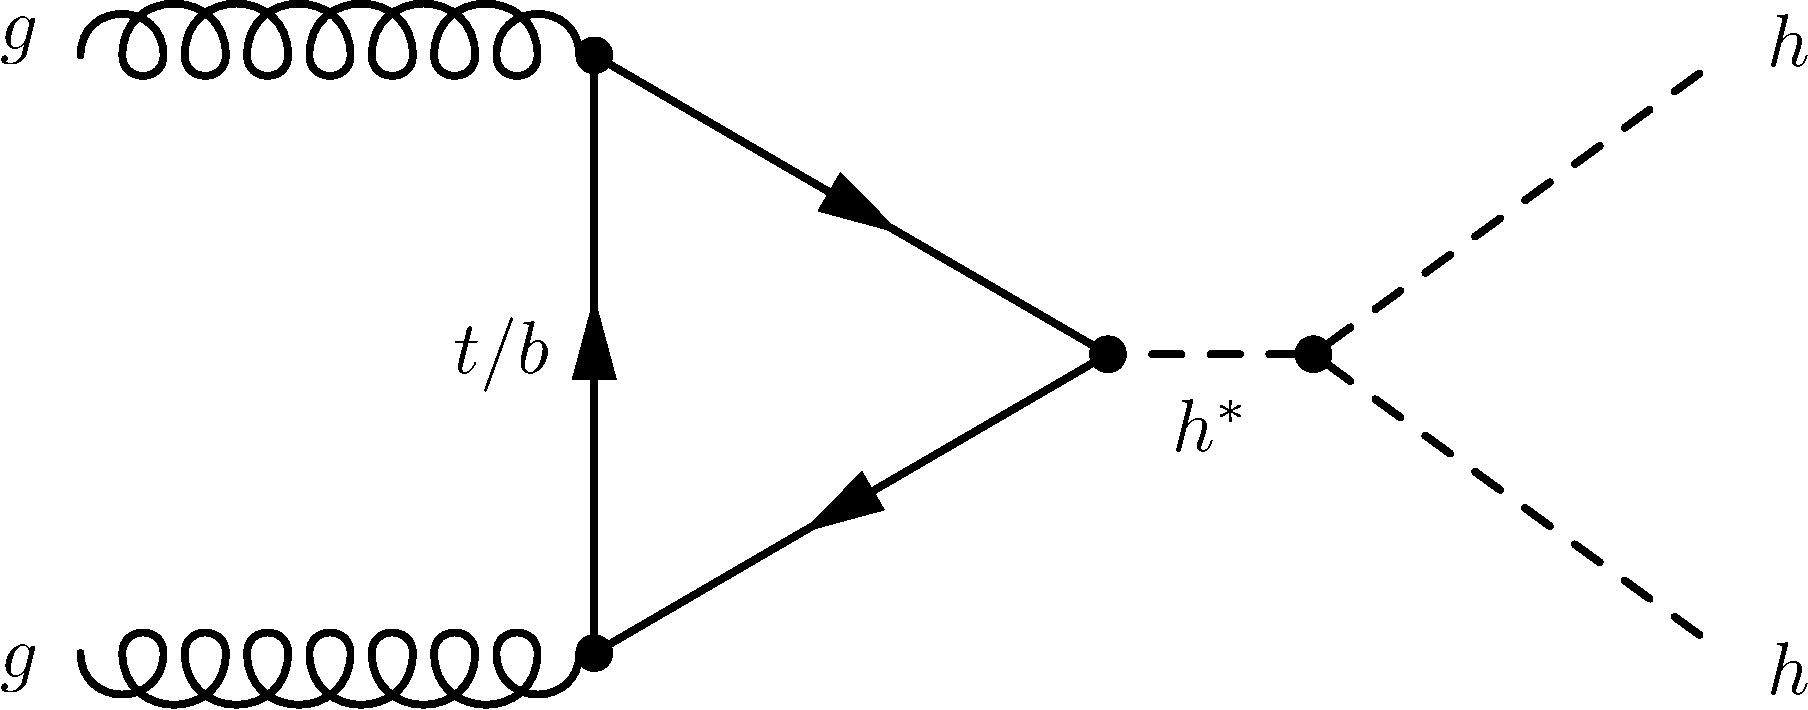
\includegraphics[width=\textwidth]{figures/theory/SM_HH_tri}
        \caption{Triangle diagram}
        \label{fig:SM_HH_tri}
    \end{subfigure}
\caption{Leading order Feynman diagrams contributing to di-Higgs production via gluon-gluon fusion, through the Higgs-fermion Yukawa interactions~\ref{fig:SM_HH_box} and the Higgs boson self-coupling~\ref{fig:SM_HH_tri}. Only Figure~\ref{fig:SM_HH_tri} probes $\lambda_{hhh}$.}
\label{fig:SM_HH}
\end{figure}

\paragraph{}
Many other different production modes of di-Higgs exist, but gluon-gluon fusion is the dominant one. Figure~\ref{fig:SM_HH_xsec}~\cite{Frederix:2014hta} compares the cross sections of gluon-gluon fusion, Vector Boson Fusion (VBF), and top-pair, $W^{\pm}$, $Z$ and single-top associated di-Higgs production.

\begin{figure}[h!]
  \centering
  \captionsetup{justification=centering}
  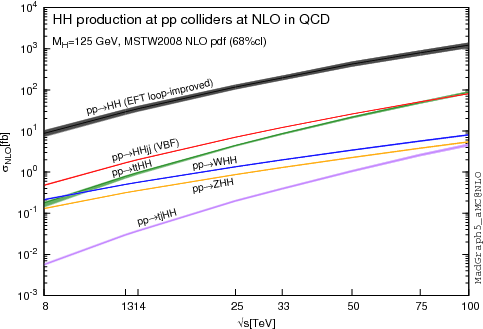
\includegraphics[width=0.7\textwidth]{figures/theory/HH_xsec}
  \caption{Total cross sections (y-axis) at the NLO in QCD for the six largest di-Higgs production channels at p-p colliders at different energy (x-axis). The thickness of the lines corresponds to the scale and PDF uncertainties added linearly. $H$ refers to the SM Higgs.}
  \label{fig:SM_HH_xsec}
\end{figure}

\paragraph{}
For p-p collisions at $\sqrt{s}=13$ \TeV, the total cross section for SM gluon fusion di-Higgs production~\cite{LHCYellow}, at the Next to Next Leading Order (NNLO) with top quark mass effects, is $33.49^{+ 4.3 \%}_{-6.0 \%} \pm 2.1\% \pm 2.3\%$ fb. The cross section for the next dominant production, VBF, is $1.62^{+ 2.3 \%}_{-2.7 \%} \pm 2.3\%$ fb. The estimated cross section for triple-Higgs production is $0.06332 ^{+ 16.1 \%}_{-14.1 \%} \pm 3.4\% $ fb, which is negligible with current dataset. The uncertainties are Scale uncertainty, PDF uncertainty and $\alpha_s$ uncertainty. This means inside 2015 and 2016 $\sqrt{s}=13$ \TeV ATLAS 36 \ifb data , there are only around one thousand SM di-Higgs events.


%%%%%%%%%%%%%%%%
\section{Beyond the Standard Model Physics di-Higgs production}
\paragraph{}
BSM physics could significantly enhance the production of di-Higgs at the LHC. This is separated into two categories: non-resonant and resonant productions. The non-resonant production generally refers to modifications of the Higgs couplings, either the Higgs self-coupling or the Higgs-top couplings. Resonant production refers to a particle with invariant mass greater than twice the Higgs mass decays directly into two Higgs bosons. The difference also comes from the distribution of the di-Higgs invariant mass at the truth level. In the non-resonant case, the distribution has no clear peak, whereas in the resonant case, the invariant mass distribution usually forms a peak with model dependent width.

\begin{figure}[h!]
\centering
\captionsetup{justification=centering}
    \begin{subfigure}[b]{0.3\textwidth}
        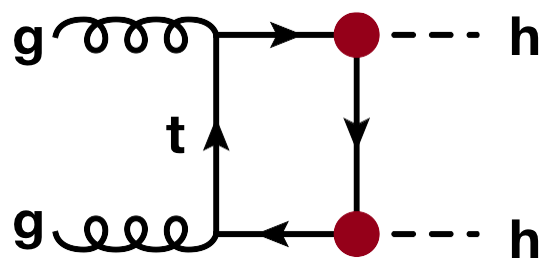
\includegraphics[width=\textwidth]{figures/theory/BSM_HH_box}
        \caption{$H$-fermion vertices variations}
        \label{fig:BSM_HH_box}
    \end{subfigure}
    \quad
    \begin{subfigure}[b]{0.3\textwidth}
        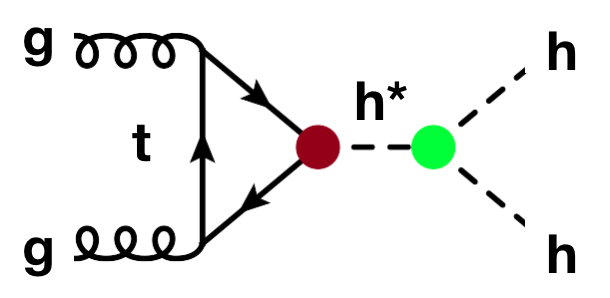
\includegraphics[width=\textwidth]{figures/theory/BSM_HH_tri}
        \caption{Higgs self-coupling variations}
        \label{fig:BSM_HH_tri}
    \end{subfigure}
    \quad
    \begin{subfigure}[b]{0.3\textwidth}
        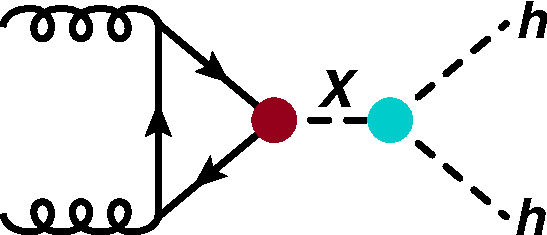
\includegraphics[width=\textwidth]{figures/theory/BSM_HH_X}
        \caption{an intermidiate resonance, X}
        \label{fig:BSM_HH_X}
    \end{subfigure}
\caption{BSM Higgs boson pair production: non-resonant production proceeds through changes in the SM Higgs couplings in~\ref{fig:BSM_HH_box} and~\ref{fig:BSM_HH_tri}, resonant production proceeds through~\ref{fig:BSM_HH_X} an intermediate resonance, X. $H$ and $h$ both refers to the SM Higgs.}
\label{fig:BSM_HH}
\end{figure}

\subsection{BSM non-resonant di-Higgs}
\paragraph{}
Enhanced non-resonant Higgs boson pair production is predicted by many models. Models featuring direct $t\bar{t}\hh$ vertices \cite{Grober:2010yv, Contino:2012xk} or new light colored scalars \cite{PhysRevD.86.095023} could change vertices shown as the red dots in Figure~\ref{fig:BSM_HH}. A direct modification of Higgs self-coupling term in Eq~\ref{eqn:higgspotential} to $\lambda hhh$, where $\lambda$ is different from $\lambda_{\rm sm}$, is also possible. This is shown as the green dot in Figure~\ref{fig:BSM_HH_tri}. 

\paragraph{}
The non-resonant di-Higgs enhancement is usually described by $\frac{\rm \lambda}{\rm \lambda_{\rm SM}}$, which is the cross section ratio between $\lambda$ and $\lambda_{\rm SM}$. From the SM electroweak measurements, the self coupling term could be constrained to $-14 \leq \frac{\rm \lambda}{\rm \lambda_{\rm SM}} \leq 17.4$~\cite{Kribs:2017znd}. Variations of $\lambda$ have a non-trivial effect on di-Higgs production cross section, shown in Figure~\ref{fig:SM_HH_lam}~\cite{Frederix:2014hta}. In the regime of relatively high trilinear coupling, the observation will be an excess of di-Higgs events with respect to the expected background. A simple limit can be set in this case.

\begin{figure}[h!]
  \centering
  \captionsetup{justification=centering}
  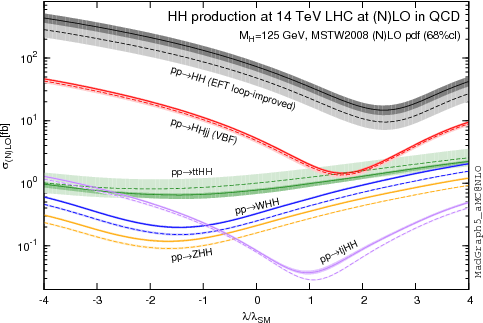
\includegraphics[width=0.7\textwidth]{figures/theory/HH_lam}
  \caption{Total cross sections (y-axis) at the LO and NLO in QCD for di-Higgs production channels, at the $\sqrt{s} = 14$ TeV LHC as a function of the self-interaction coupling $\lambda$ (x-axis) . The dashed (solid) lines and light- (dark-) color bands correspond to the LO (NLO) results and to the scale and PDF uncertainties added linearly. The SM values of the cross sections are obtained at $\frac{\rm \lambda}{\rm \lambda_{\rm SM}} = 1$. $H$ refers to the SM Higgs.}
  \label{fig:SM_HH_lam}
\end{figure}

\subsection{BSM resonant di-Higgs}
\paragraph{}
Resonant Higgs boson pair production is also predicted by many models. Extensions of the Higgs sector, such as two-Higgs-doublet models(2HDM)~\cite{PhysRevD.8.1226, Branco:2011iw}, propose the existence of a heavy spin-0 scalar $H$ that can decay into di-Higgs. The bulk Randall-Sundrum model~\cite{Agashe:2007zd, Fitzpatrick}, which features spin-2 Kaluza-Klein gravitons, \Grav, could also subsequently decay to pairs of Higgs bosons. These proposed heavy particles, heavy CP-even scalar $H$ and \Grav, are represented as X in Figure~\ref{fig:BSM_HH_X}.

\paragraph{}
The 2HDM is a a simple extension of the SM which can exhibit large resonance effects~\cite{LHCYellow}. The 2HDM has 5 physical Higgs bosons: $h$ (light scalar Higgs), $H$ (heavy scalar Higgs), $A$ (heavy pesudoscalar Higgs), and $H^{\pm}$ (two charged Higgs). The 2HDM can introduce tree level favor changing neutral currents. To avoid this, models impose discrete symmetries in which the charged fermions only couple to one of the Higgs doublets. One version is type II 2HDM, in which all positively charged quarks couple to one doublet and the negatively charged quarks and leptons couple to the other. The type II model is the Minimal Supersymmetric Standard Model(MSSM)'s Higgs sector.

\paragraph{}
Resonant di-Higgs production in 2HDM models can proceed through decays of the heavy CP-even Higgs $H\to hh$. The branching ratio for $H\to hh$ depends on the model type as well as the values of $\tan{\beta}$ and $\cos(\beta - \alpha)$. $\tan{\beta} = \frac{\rm \nu_{\rm doublet2}}{\rm \nu_{SM}}$ is the ratio of the vacuum expectation values of the two Higgs doublets. $\alpha$ is the mixing angle between the heavy $H$ and light $h$ fields. The limit where $\cos(\beta - \alpha) = 0$ is called the alignment limit, and in this limit the light Higgs $h$ has the same couplings as a SM Higgs. Near the alignment limit there is some unprobed phase space depending on the exact models and values of $\tan{\beta}$ being considered, and they are particulary interesting to be searched for at the LHC.


\paragraph{}
The Randall-Sundrum model proposes a five-dimensional warped spacetime that contains two manifolds: one where the force of gravity is very strong and a second manifold at the \TeV scale corresponding to the known SM sector. The experimental consequence of this theory is a series of widely spaced (in mass) Kaluza-Klein graviton resonances, \Grav. In theories where the fermions are localized to the SM brane, production of gravitons from fermion pairs is suppressed and the primary mode of production is gluon fusion. These gravitons have a substantial branching fraction to di-Higgs, ranging from $6.43$\% for gravitons with a mass of $500$ \GeV to $7.66\%$ at $3$ \TeV. Randall-Sundrum models have two free parameters - the mass of the graviton and $c = k/\bar{M}_{\rm pl}$, where $\bar{M}_{\rm pl}$ is the reduced Planck mass and $k$ is the curvature parameter. The width of the graviton increases with both mass and $c$.

\begin{figure}[h!]
  \centering
  \captionsetup{justification=centering}
  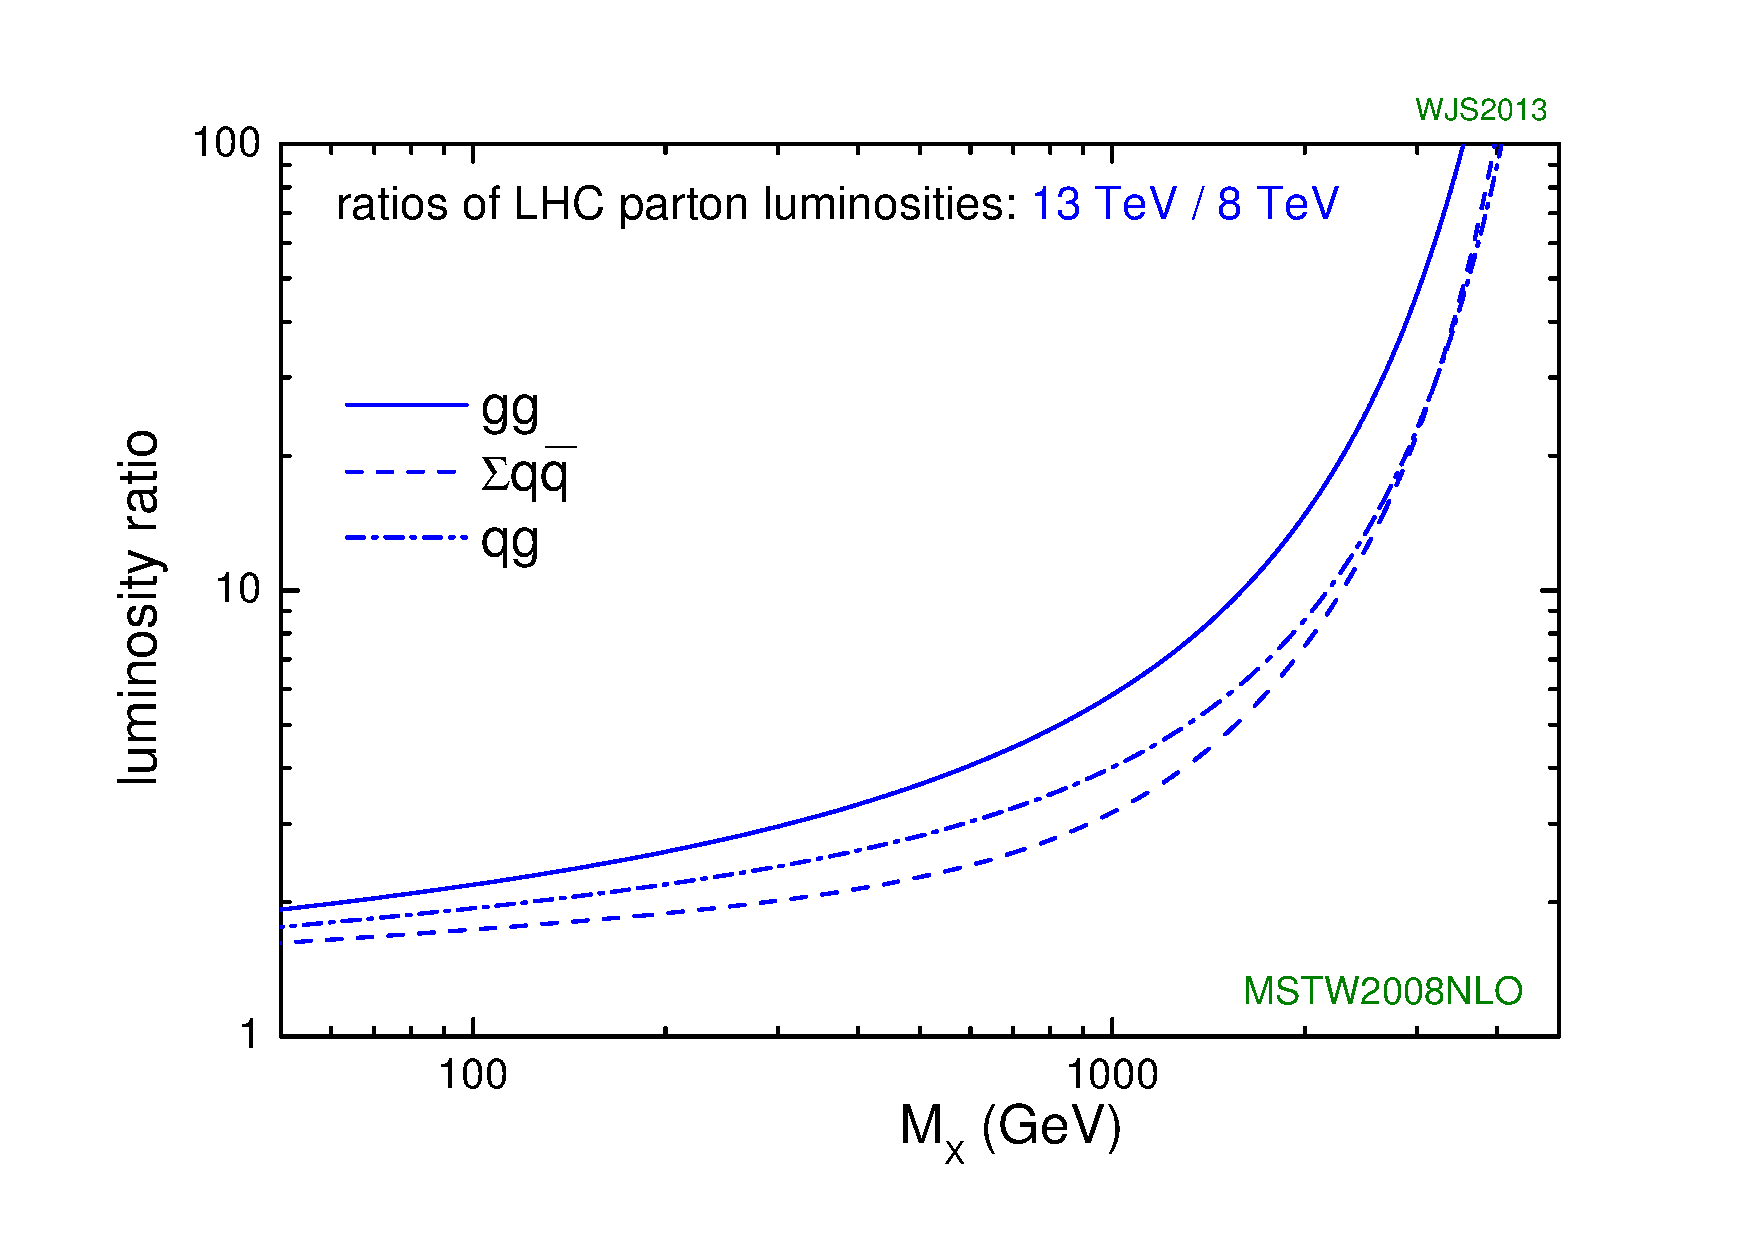
\includegraphics[width=0.7\textwidth,angle=270]{figures/theory/lhclumi7813_2013_v1.pdf}
  \caption{Parton luminosity ratios as a function of resonance mass $M_{X}$ for $13/8$ \TeV~\cite{LumiRatio}. For a $2$ \TeV $X$, the lumniosity ratio is almost 10.}
  \label{fig:lumi_ratio}
\end{figure}

\paragraph{}
%In summary, resonant di-Higgs searches could test many models including extra dimensions and Supersymmetry. 
Generally, it is easy theoretically for new heavy resonance particles to interact with the SM through the Higgs as a portal, resulting in resonance di-Higgs production. With the increased center of mass collision energy from $8$ \TeV~ to $13$ \TeV, the production cross section through gluon-gluon fusion for heavy particles above \TeV~ grows in LHC Run 2, as shown in Figure~\ref{fig:lumi_ratio}. Therefore, it is particularly important to focus on resonant searches above \TeV~ region.


\section{Di-Higgs Decay and LHC previous search results}
\paragraph{}
Di-Higgs decay is a combination of single Higgs decays. The coupling terms to fermions and bosons are shown in Eq~\ref{eqn:higgspotential}. The branching ratio of the di-Higgs final state is shown in Figure~\ref{fig:HH_BR}.

\begin{figure}[h!]
  \centering
  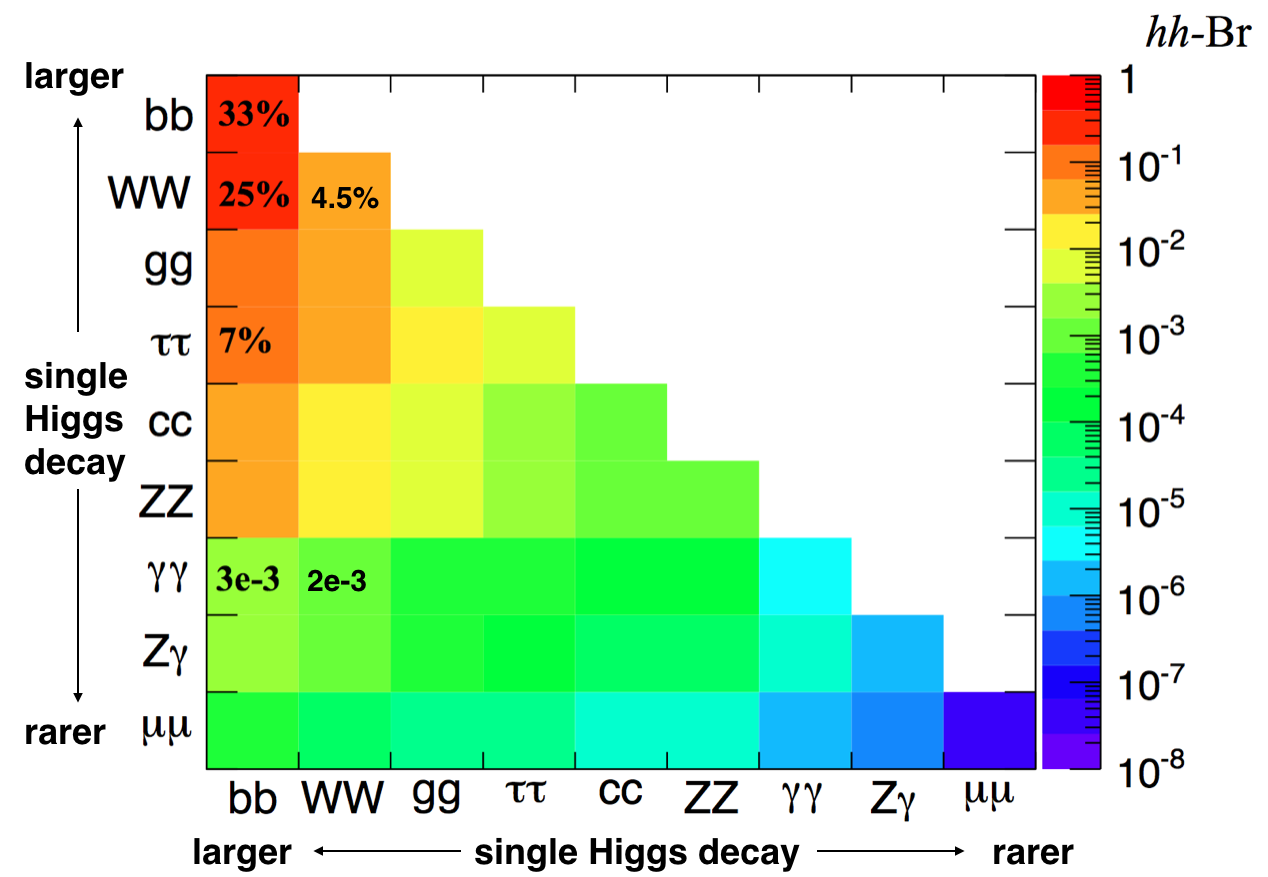
\includegraphics[width=0.7\textwidth]{figures/theory/HH_BR}
  \caption{Summary of di-Higgs final states and their ratios. Top left, \bbbb, has the largest branching ratio.}
  \label{fig:HH_BR}
\end{figure}

\paragraph{}
Previous searches for Higgs boson pair production have all yielded null results. Using 8~\TeV\ data, ATLAS has examined the \bbbb~\cite{Aad:2015uka}, \bbgg~\cite{HIGG-2013-29}, \bbtautau and \WWgg~ channels, all of which were combined in Ref~\cite{Aad:2015xja}. The resonant search combination result is shown in Figure~\ref{fig:Run1_ATLAS}. The best non-resonant $\sigma(pp \to hh)$ cross section limit in Run 1 is the ATLAS combination, at $0.69$ pb. This crossponds to $\frac{\rm \lambda}{\rm \lambda_{\rm SM}} <70$. Different di-Higgs search challenges and perspectives are summarized below:
\begin{itemize}
	\item \bbbb~: Trigger limits the low mass resonance searches, but for high mass resonances above 500 \GeV, the branching ratio of this channel provides a decisive advantage. Great for non-resonant searches.
	\item \bbWW: Despite the second largest branching ratio, large background from \ttbar~ limits this search sensitivity.
	\item \bbgg~: Benefit from a good double photon trigger efficiency, a good photon reconstruction efficiency and a low SM background. Most sensitive at low mass $m_{X} \leq 350$ \GeV. At higher masses, the smaller branching ratio and the merging of photons hurt the search sensitivity. Great for non-resonant searches.
	\item \bbtautau~: An intermediate choice between \bbbb~ and \bbgg~ for resonance searches. Yet this channel contributes to the non-resonant result significantly.
	\item \WWgg~: Suffers from much lower branching ratio and lower reconstruction efficiency of the $W^+W^-$ compared to $b\bar{b}$.
	\item $W^+W^-\tau\tau$, $W^+W^-W^+W^-$, $b\bar{b}ZZ$: There are no search results on these channels yet. But because of the relatively large branching ratio, it is likely that they would be explored in the future.
\end{itemize}

\begin{figure}[h!]
  \centering
  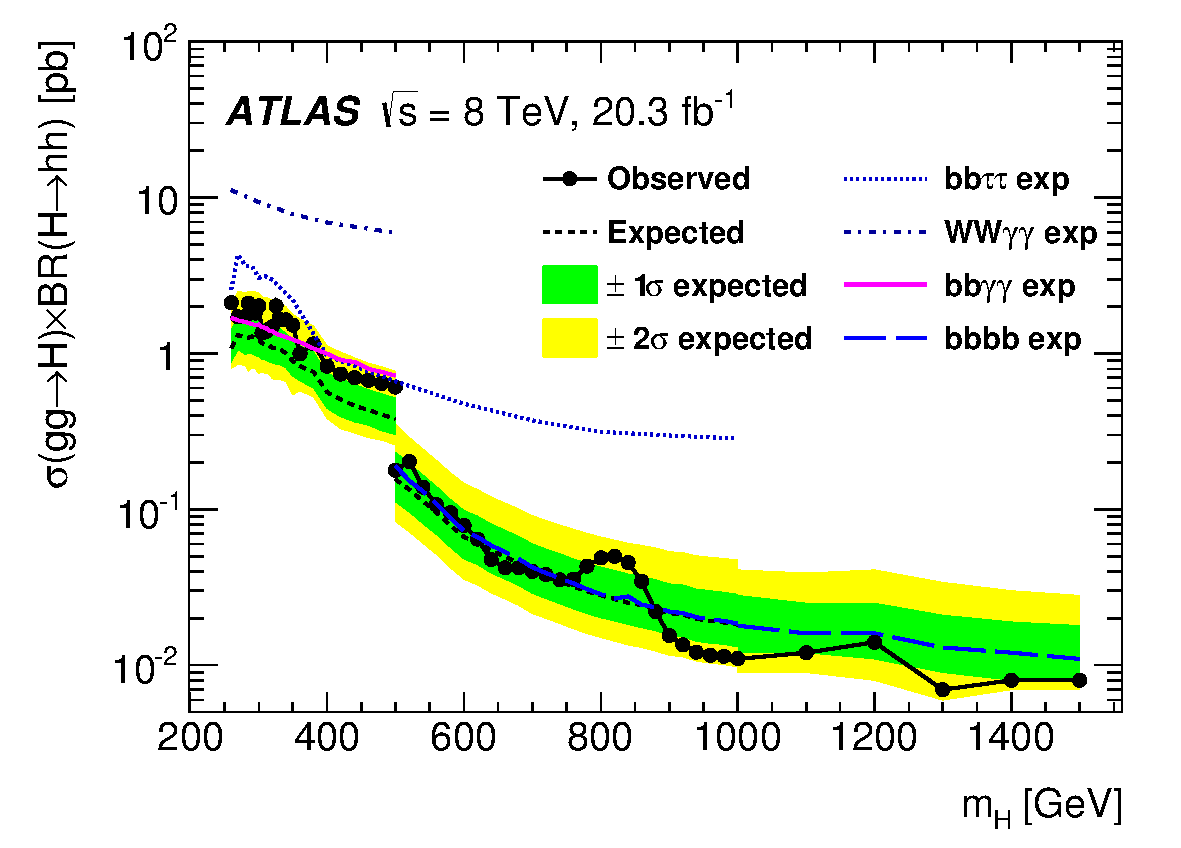
\includegraphics[width=0.7\textwidth]{figures/theory/Run1_ATLAS}
  \caption{The observed and expected 95$\%$ CL upper limits of $\sigma(gg \to H) \times BR(H \to hh)$ at $\sqrt{s}=8$ \TeV as functions of the heavy Higgs boson mass $m_{H}$, combining resonant searches in Higgs boson pair to \bbtautau~, \WWgg~, \bbgg~, and \bbbb~ final states. The expected limits from individual searches are also shown. The green and yellow bands represent $\pm 1\sigma$ and $\pm 2\sigma$ uncertainty ranges of the expected combined limits. The improvement above $m_{H} =500$ GeV reflects the sensitivity of the \bbbb~ analysis. The results beyond 1 \TeV are only from the \bbbb~ final state alone.}
  \label{fig:Run1_ATLAS}
\end{figure}

\paragraph{}
In summary, di-Higgs has a small production rate in the SM, but could be significantly enhanced in BSM scenarios. In particular, a heavy resonance spin-0 or spin 2 particle could decay into Higgs boson pair directly. The search sensitivity for resonance mass above \TeV~ increases as the center of mass energy of the collision increases. For resonance signals above 1 \TeV~ decaying into di-Higgs, \bbbb~ channel has the best discovery potential in Run 2. Therefore, searching for \TeV~ scale resonance production of di-Higgs $\to$ \bbbb~ is the goal of thesis.
% In LHC Run 2, in the \bbbb~channel, ATLAS searched for both non-resonant and resonant production in the mass range of 400--3000~\GeV\ using 3.2 $\mathrm{fb}^{-1}$ of 13~\TeV\ data~\cite{EXOT-2015-11} collected during 2015.


